\documentclass{article}
\usepackage[a4paper, tmargin=1in, bmargin=1in]{geometry}
\usepackage[utf8]{inputenc}
\usepackage{graphicx}
\usepackage{parskip}
\usepackage{pdflscape}
\usepackage{listings}
\usepackage{hyperref}


\title{CS 663 Project - Document Scanner}
\author{Meet Udeshi - 14D070007\\
Arka Sadhu - 140070011\\
Sravan Patchala - 14D070012\\
}
\date{November 2016}

\begin{document}
\maketitle
 
\section*{Problem Statement}

We capture parts of a document, with overlapping regions between the images and then reconstruct the  whole document by stitching the images.

\section*{Experimental Results}
\subsection*{Image Poster}

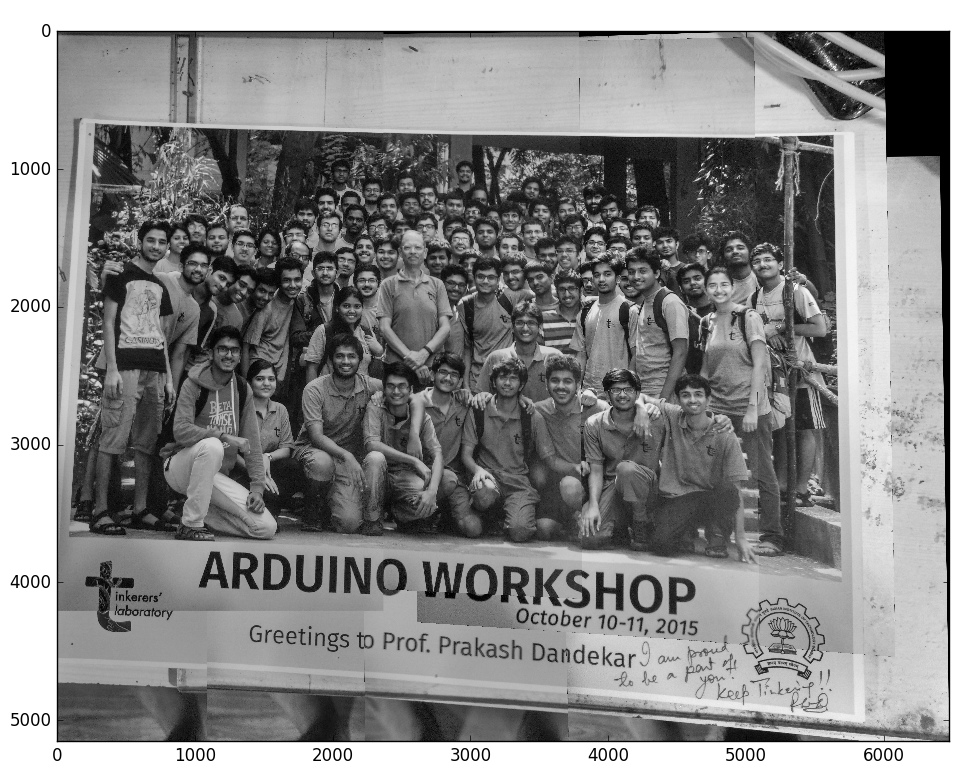
\includegraphics[scale=0.25]{tl_poster/figure_1}
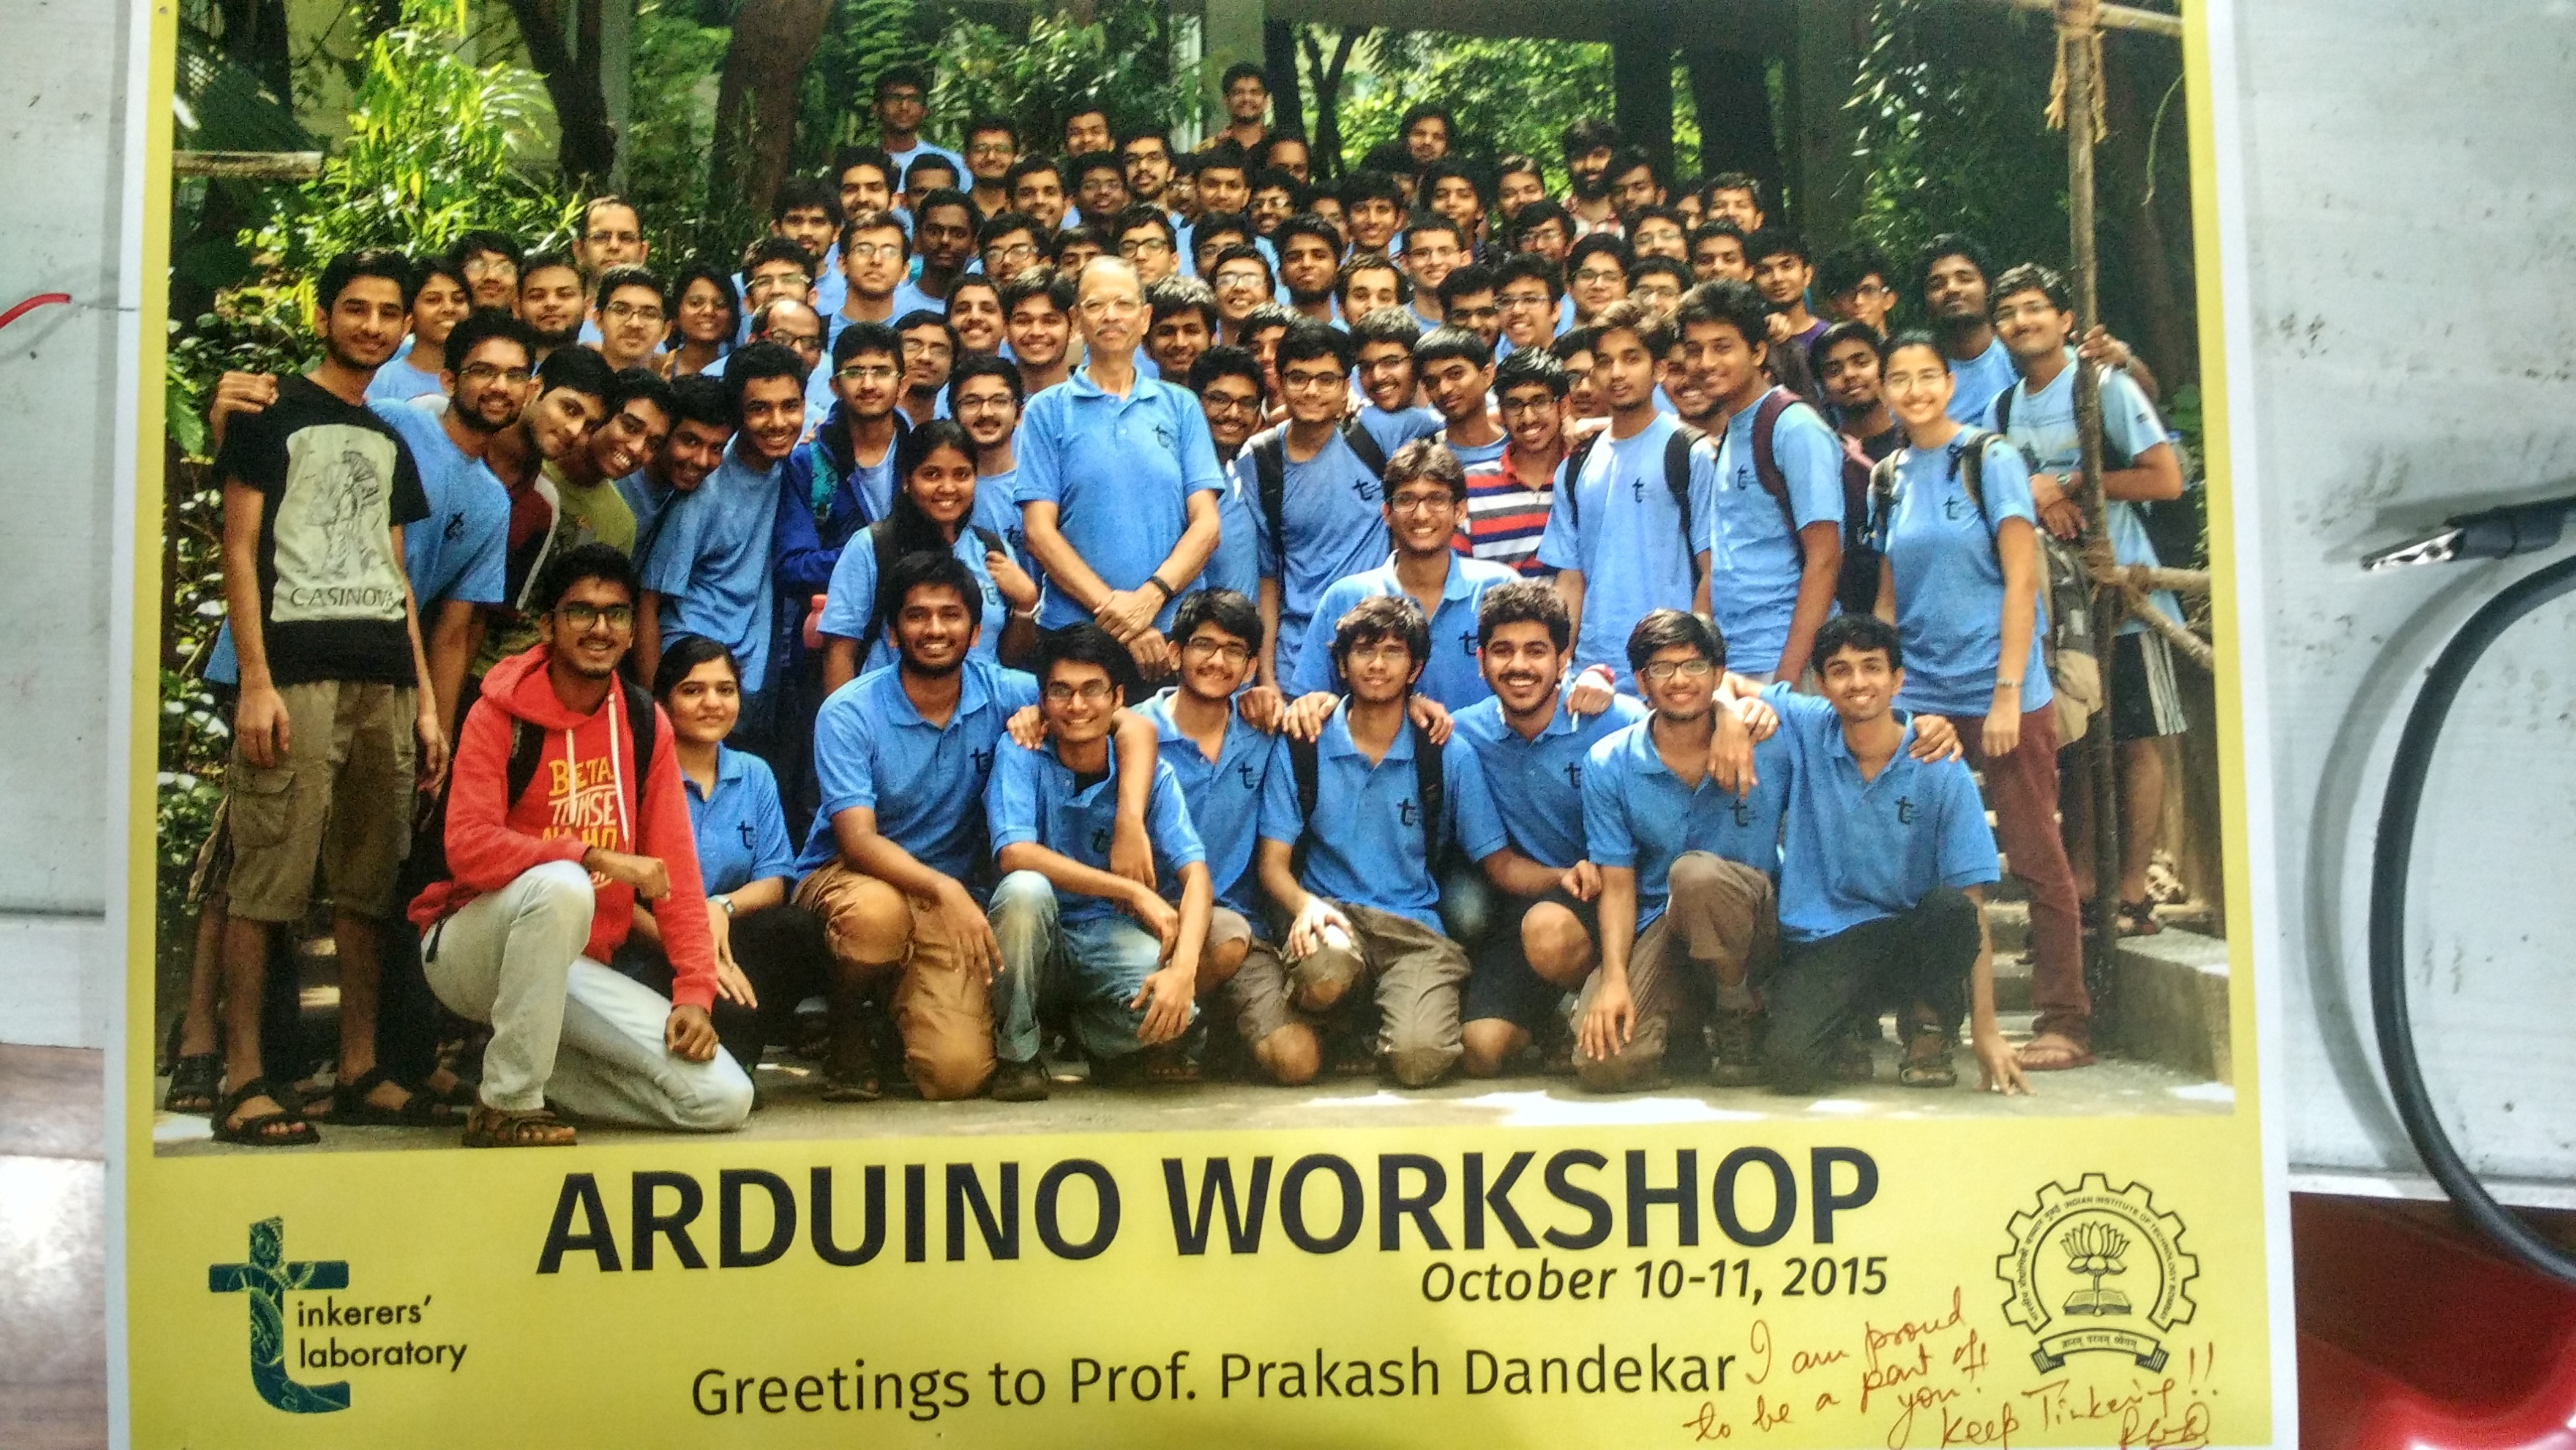
\includegraphics[scale=0.075]{tl_poster/original_tl_poster}

\subsection*{Poster with Image and Text}
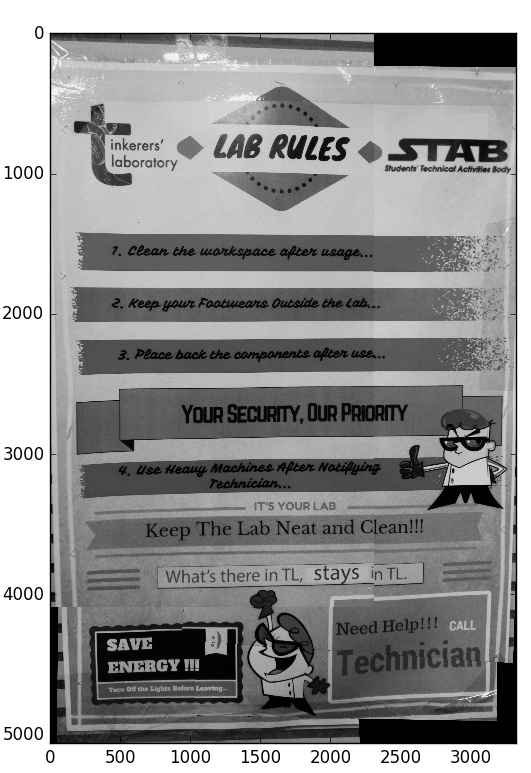
\includegraphics[scale=0.25]{lab_rules/figure_1}
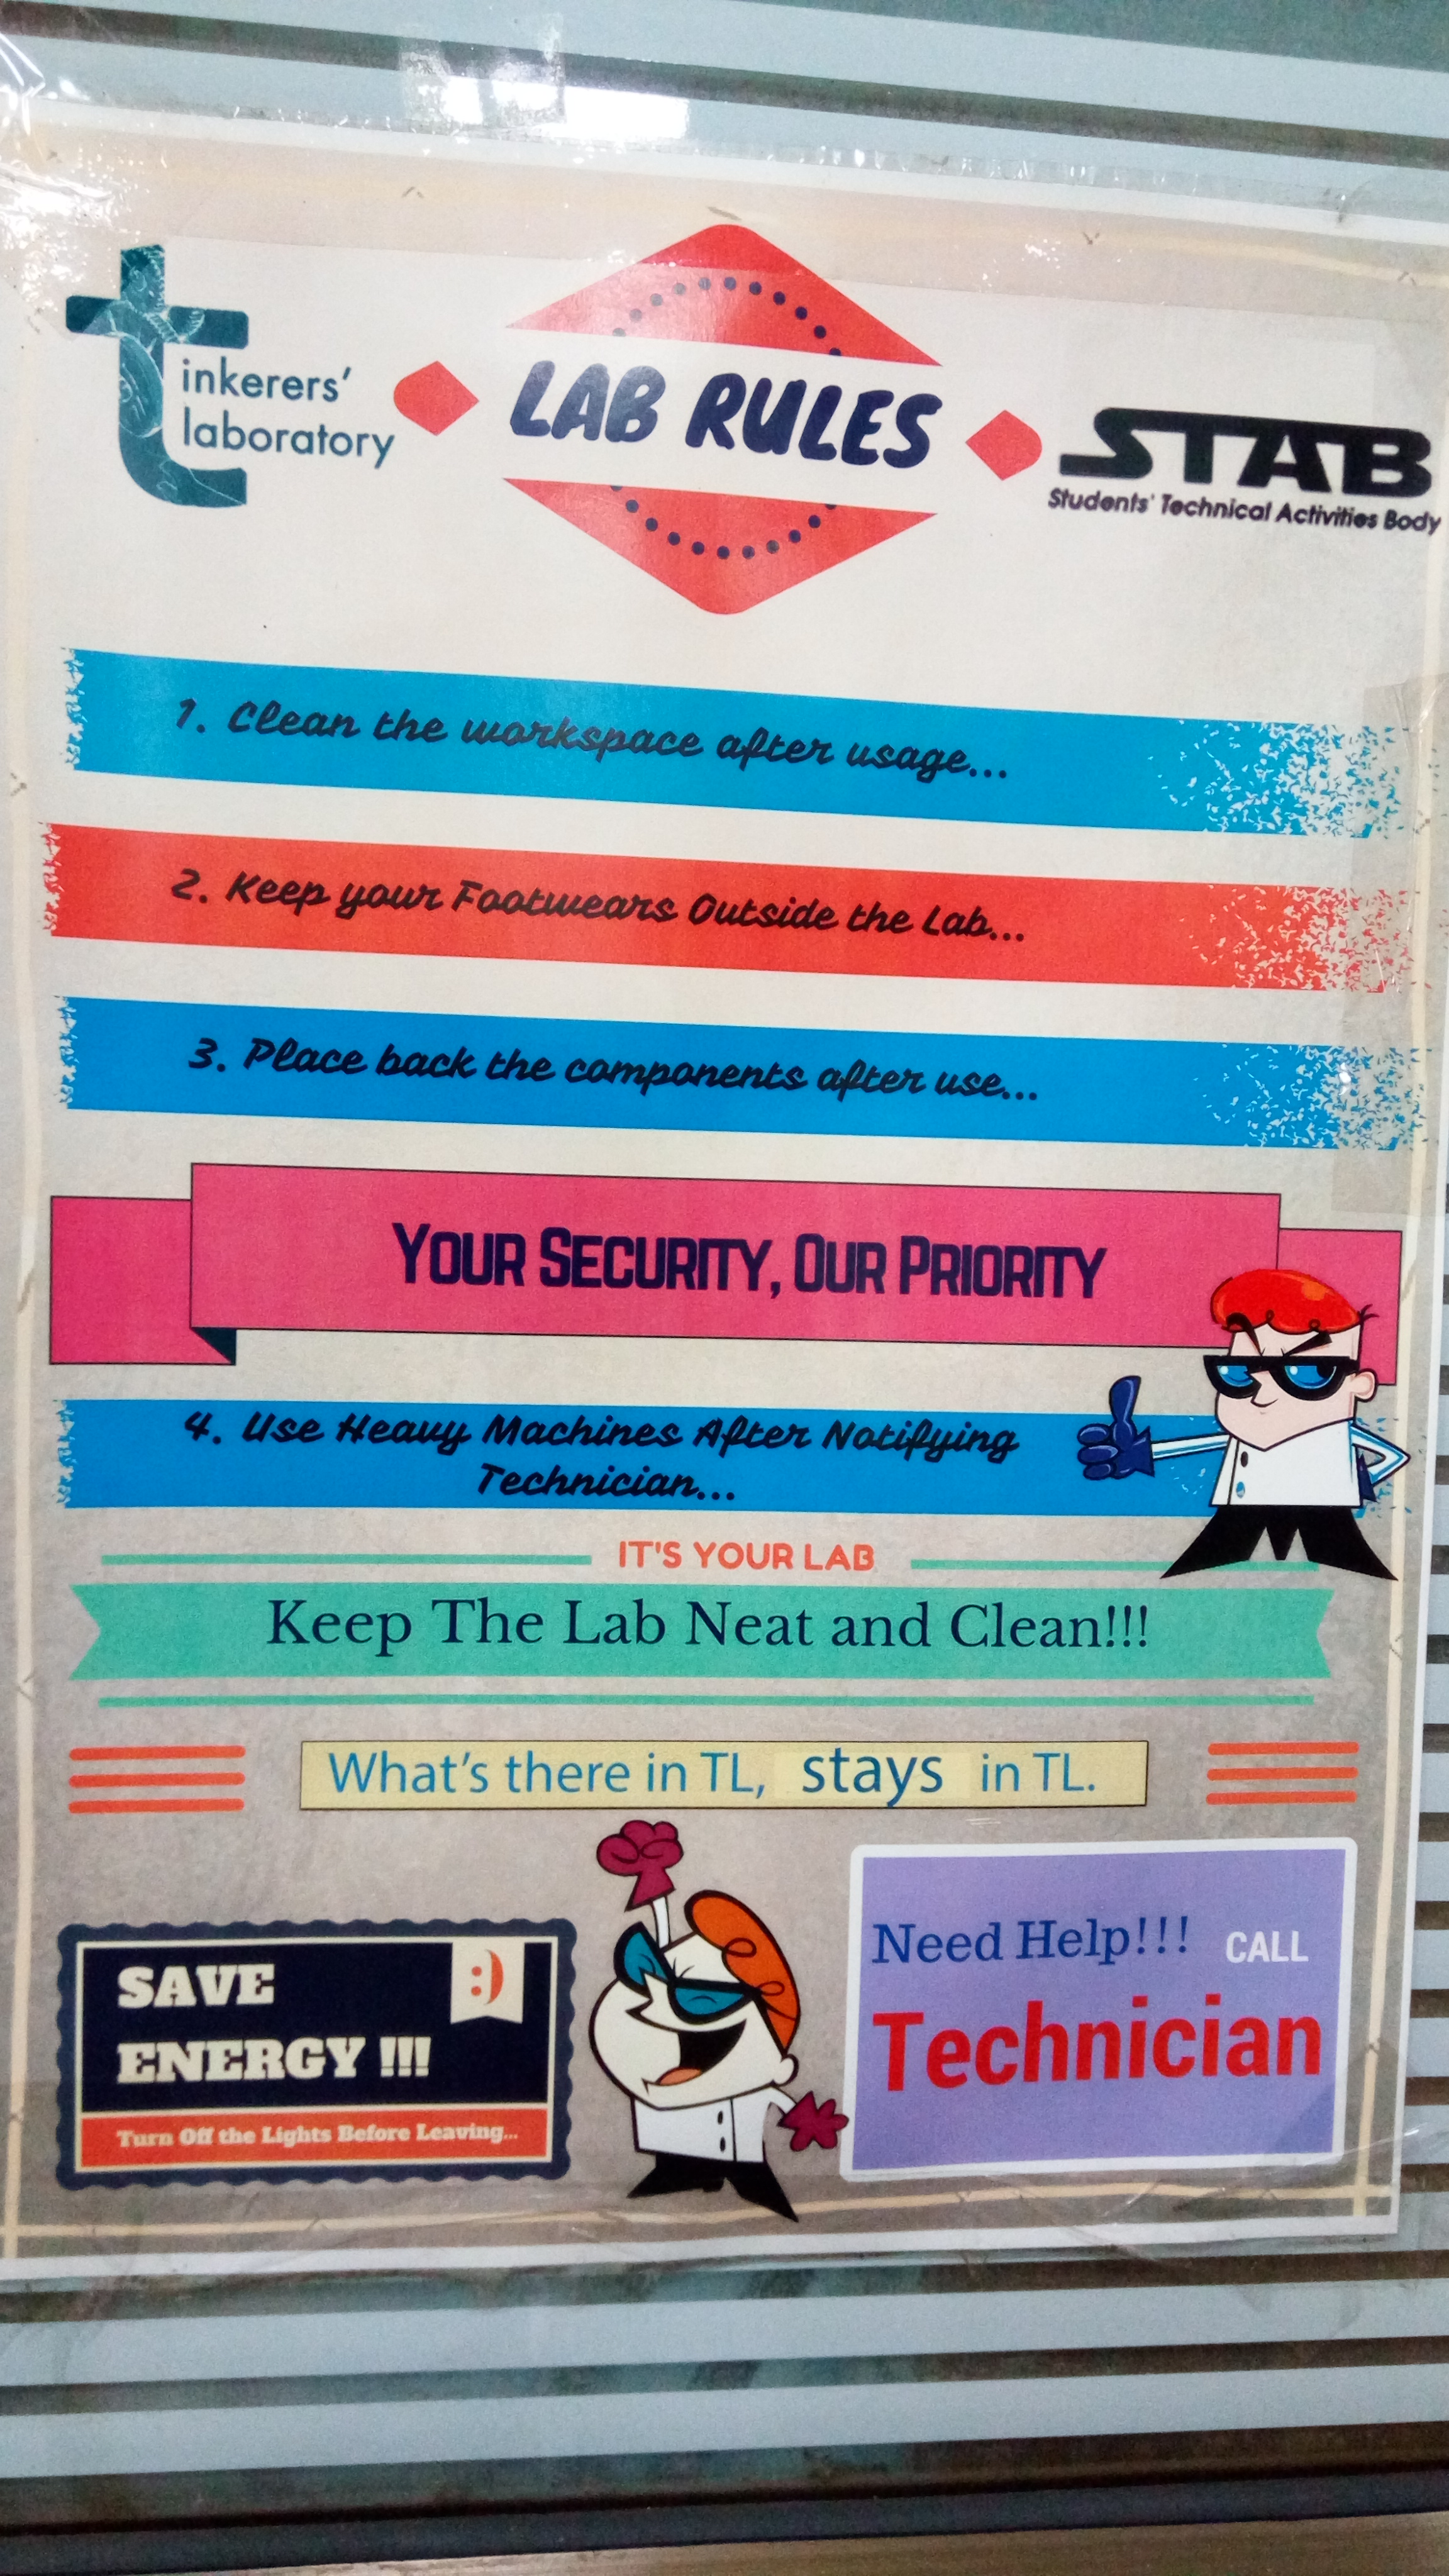
\includegraphics[scale=0.05]{lab_rules/original_lab_rules}

\subsection*{White Text on Dark Background}

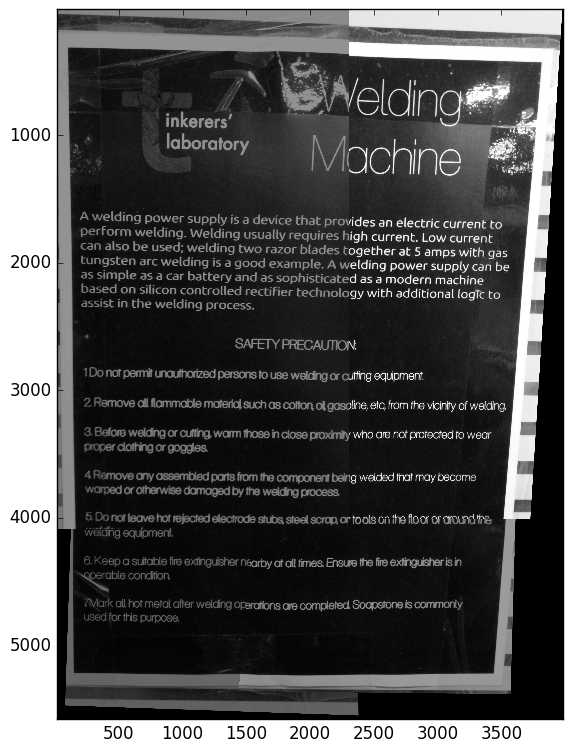
\includegraphics[scale=0.25]{welding_machine/figure_1}
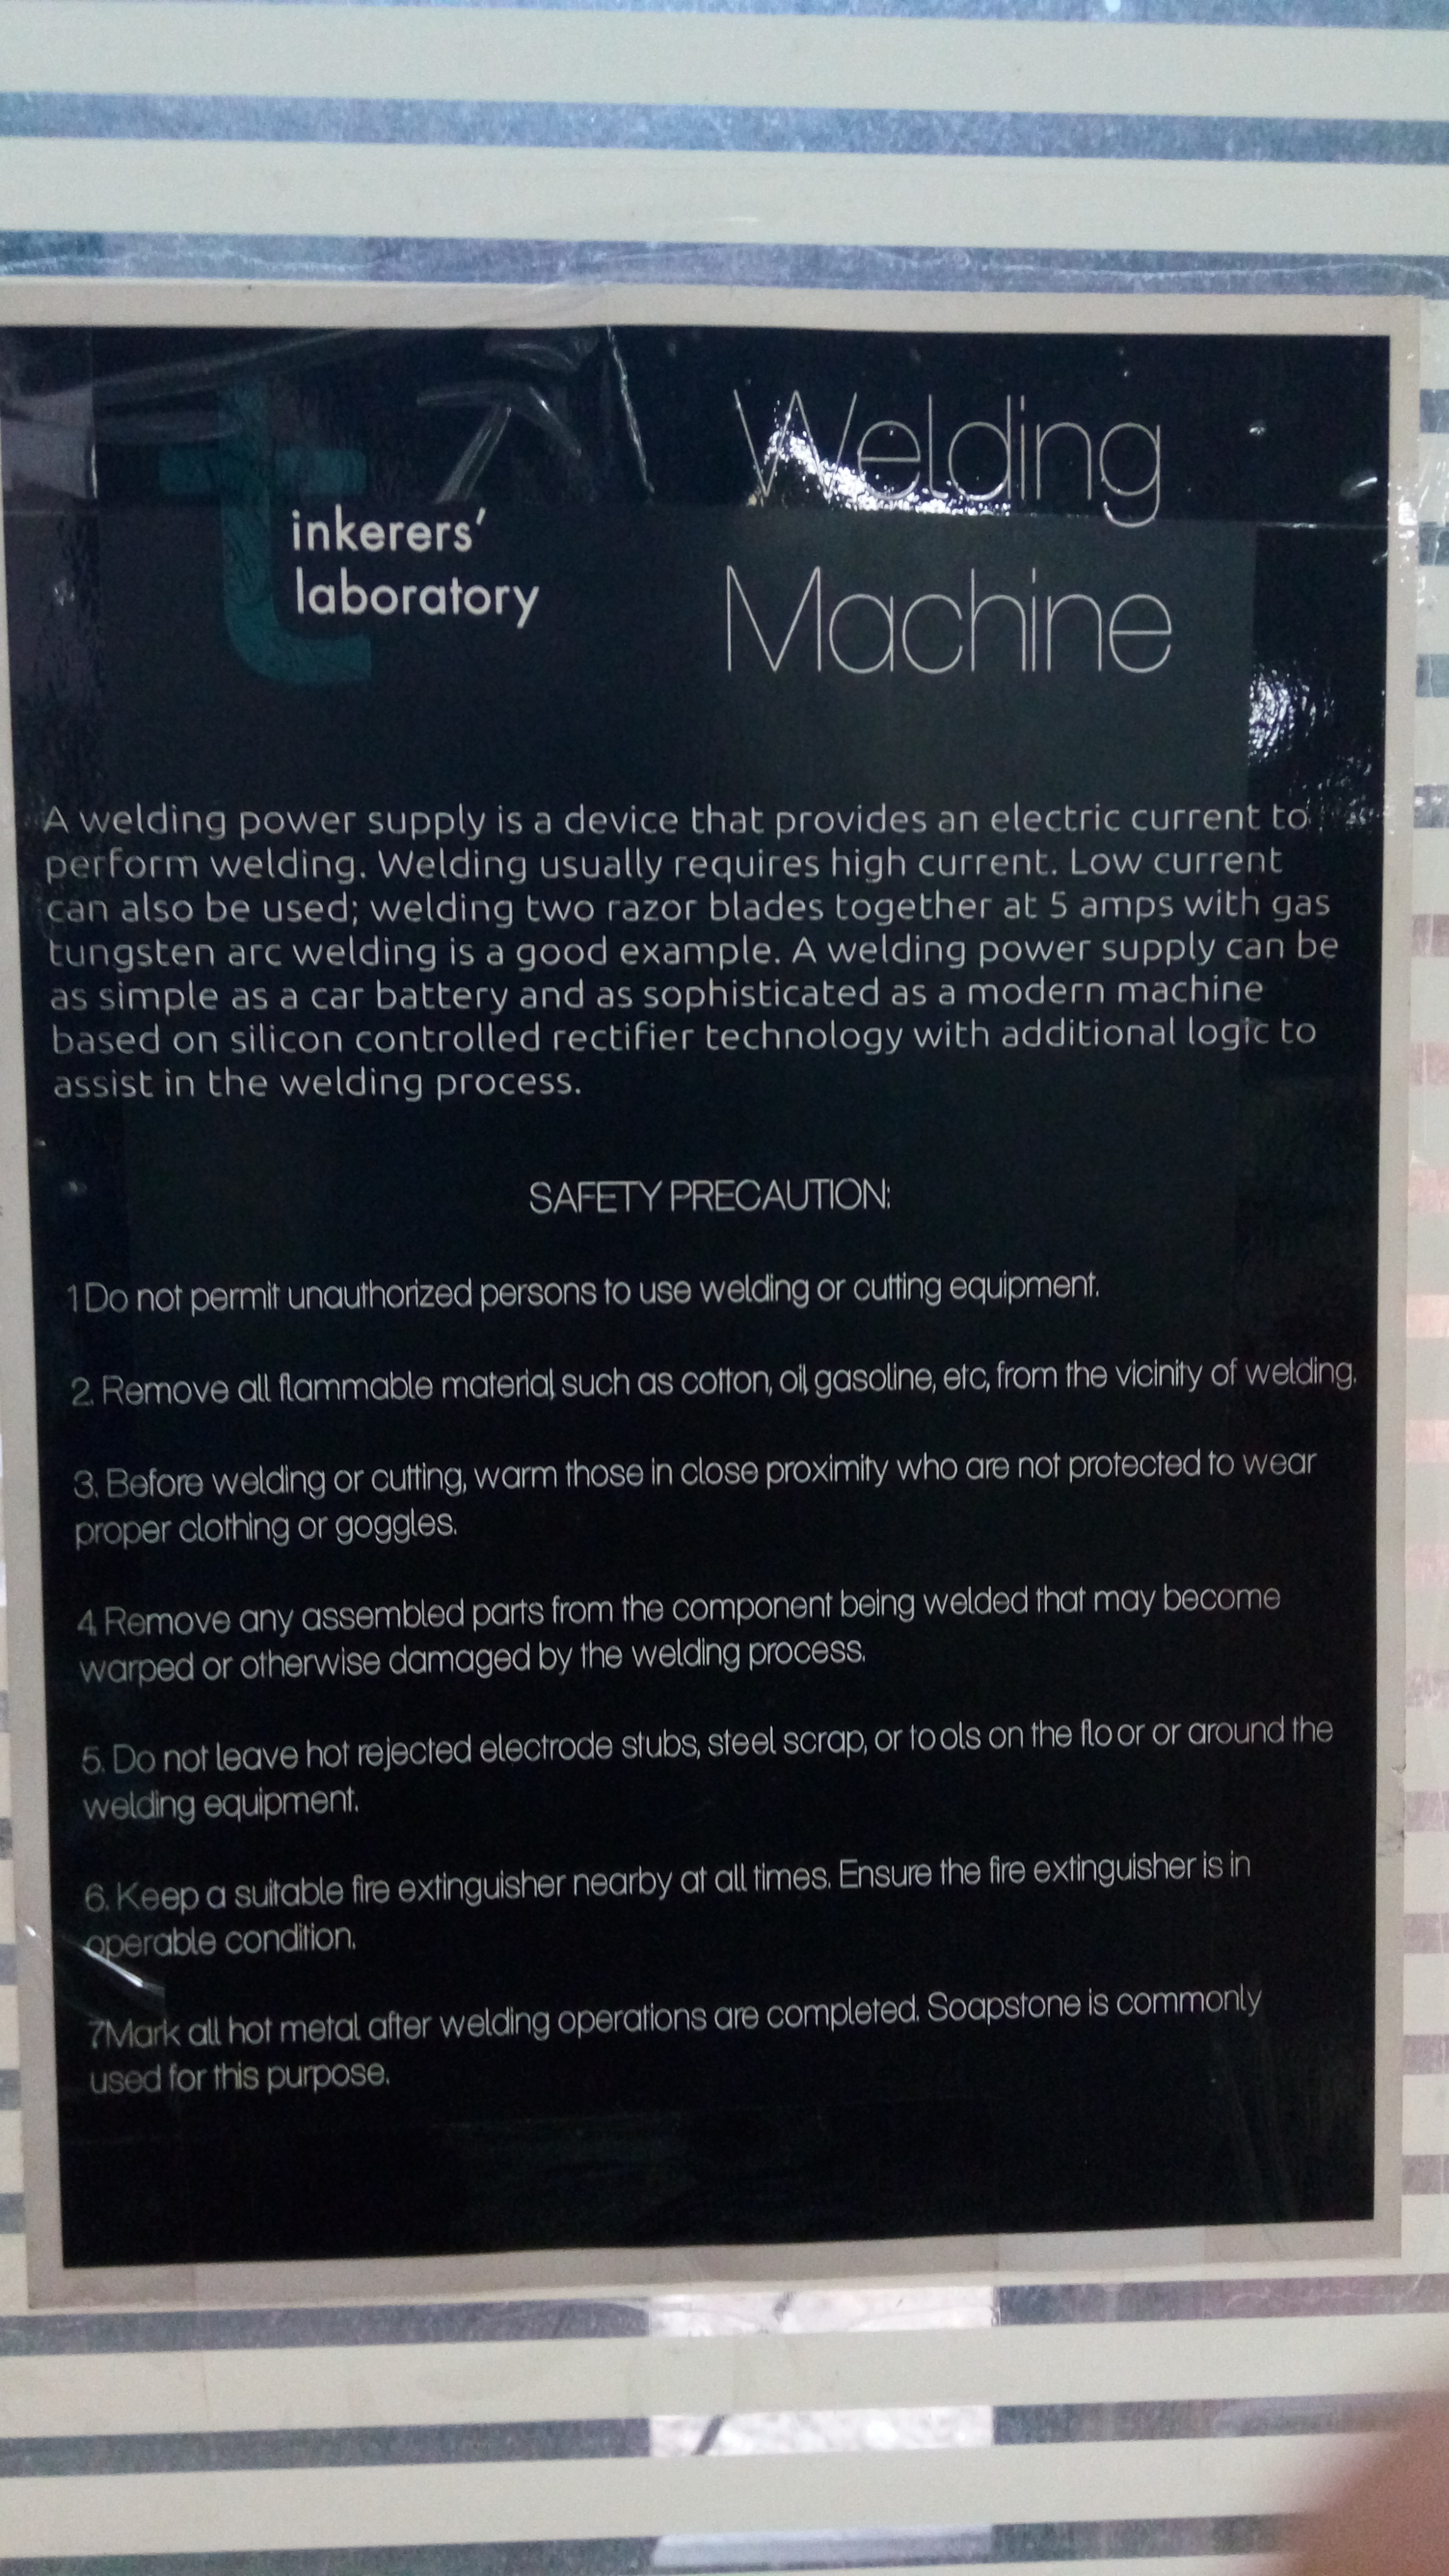
\includegraphics[scale=0.05]{welding_machine/original}

\subsection*{Multiple Posters with both text and images}

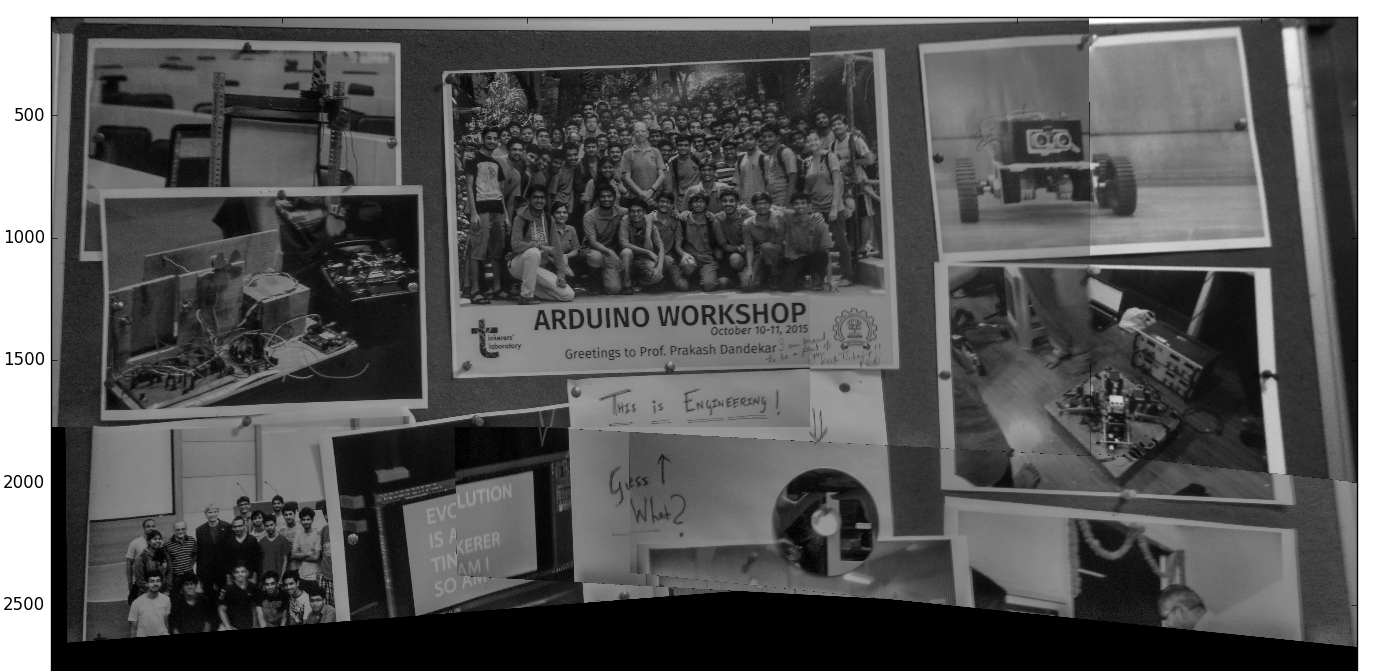
\includegraphics[scale=0.25]{softboard/figure_1}

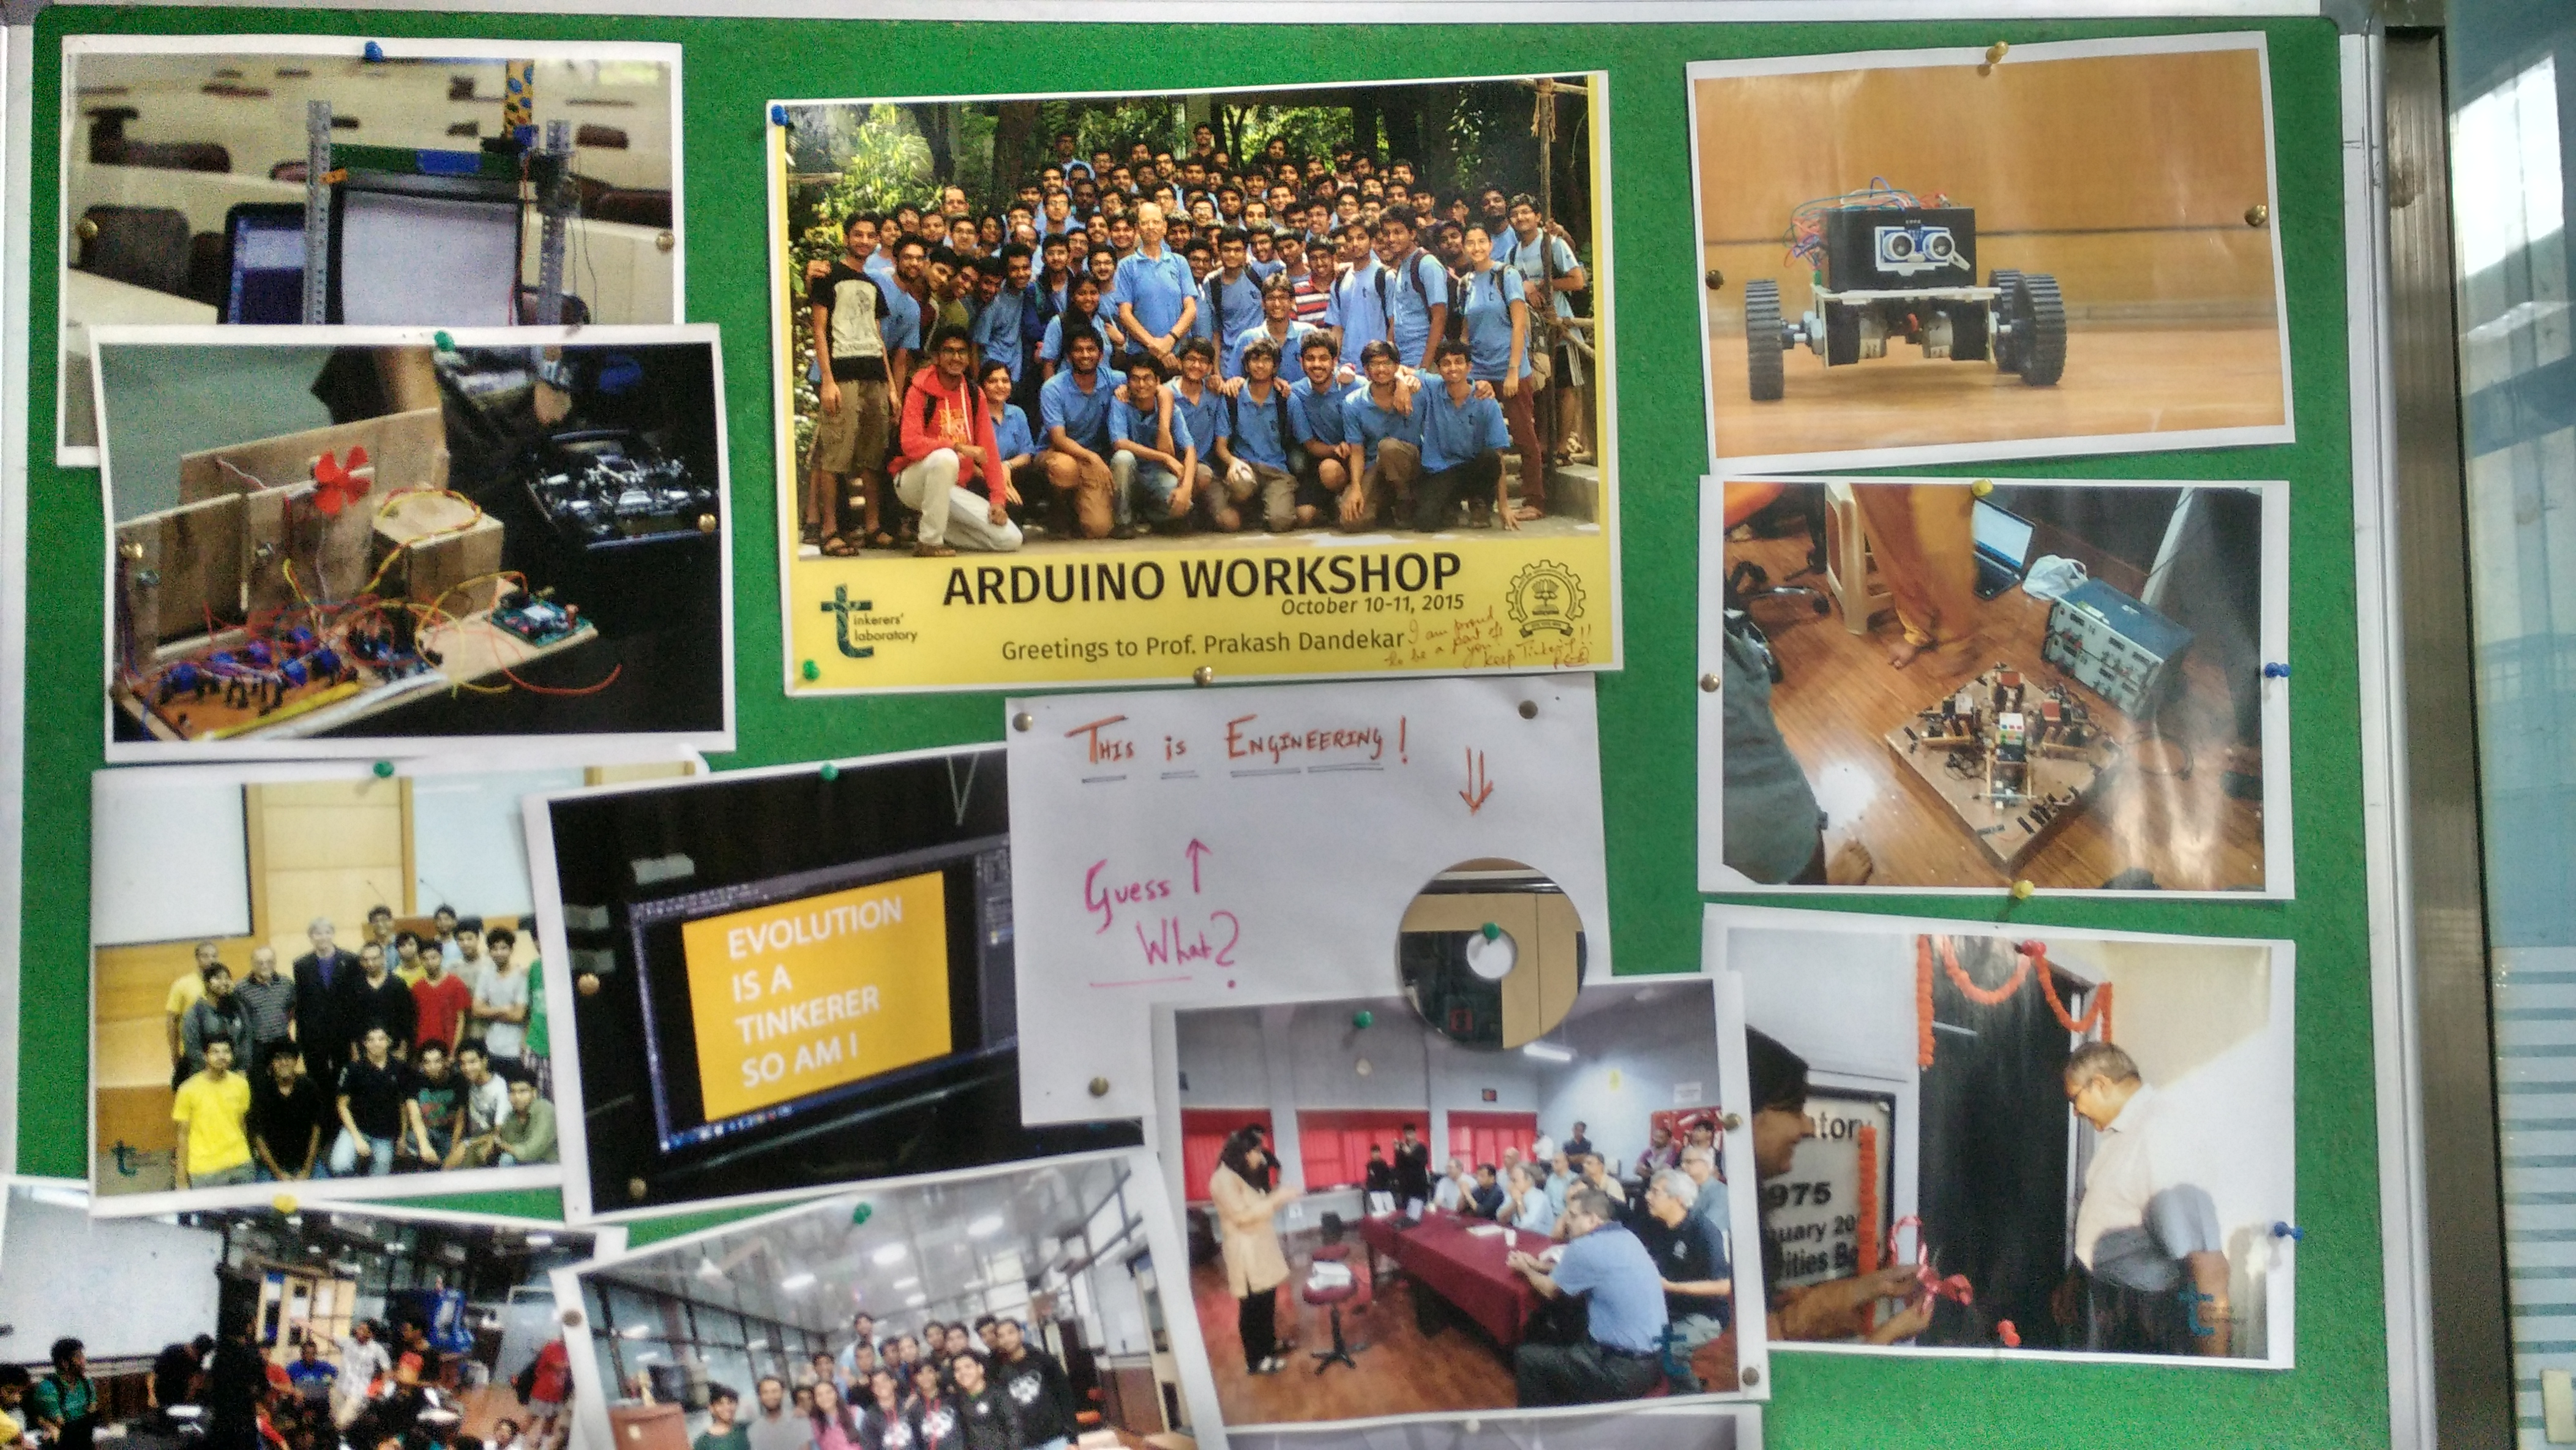
\includegraphics[scale=0.1]{softboard/original}

\subsection*{Printed text document with images}

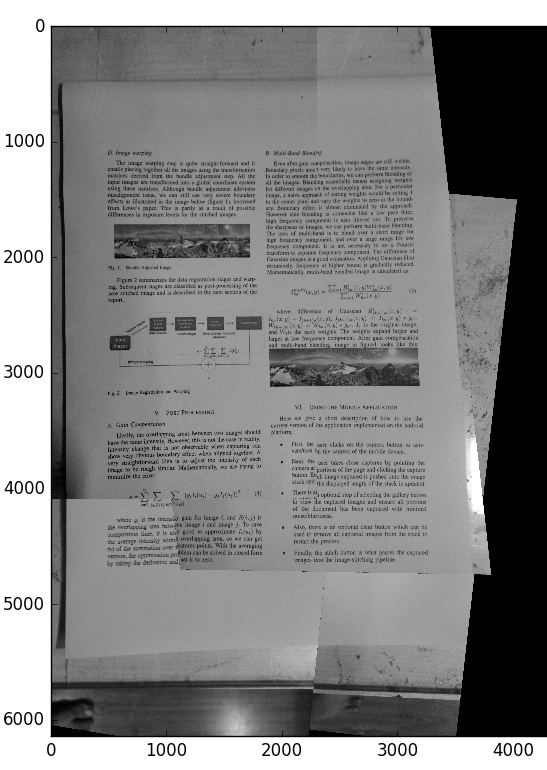
\includegraphics[scale=0.25]{badlani/figure_1}
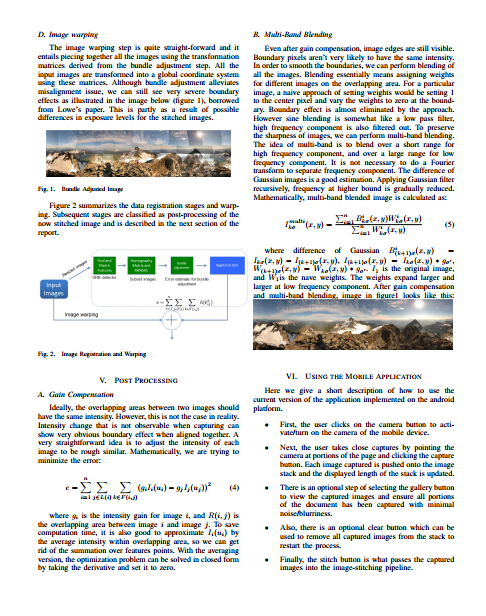
\includegraphics[scale=0.3]{badlani/original}

\section*{Procedure}

\subsection*{Procedure described in the paper 
\href{https://stacks.stanford.edu/file/druid:bf950qp8995/Badlani_Akinola_Li.pdf}{Badlani Akinola}}

\begin{itemize}
\item Feature Matching
\item Homography Matrix computation using RANSAC
\item Bundle Adjustment
\item Gain Compensation
\item Multi-Band Blending
\end{itemize}

\subsection*{What We Have Implemented}

\begin{itemize}
\item We have successfully implemented Feature Matching. We used ORB feature detection function inbuilt in OpenCV Python.
\item Next we  implemented RANSAC on our own. 
\item We adjusted the parameters in probabilistic modelling to get the correct number inliers
\item We experimented with different ways to merge the image. We tried simple merging, and then merging sequentially. The latter gave much better homographies.
\item We tried doing Bundle Adjustment. There is no direct implementation in OpenCV Python, so we created our own Bundle Adjuster. But this doesn’t give much better results compared to normal merging, so we are not using this in the final code. Also scipy cannot be ported to Android so we did not go much further with it.
\item We implemented gain compensation.
\item We also implemented Multi-Band Blending using laplacian pyramids
\end{itemize}

\subsection*{Interesting Observations}

We did the following changes from the paper:

\begin{enumerate}

\item We are calculating homography after scaling down. But we can’t directly apply to the original image. Applying this to the original image and then upsampling will cause a lot of errors. So instead we find the equivalent Matrix Transformation $S * H * S^{-1}$. This causes no error due to discretization.

\item We also tried out Image Merging by adding image one by one. We are doing this by maintaining a queue. So suppose Image2 matches with Image1, then we  compare Image3 with the composite Image2 and Image1, this returns much better result than the one got by simple merging by projecting everything to Image 1.

\item We experimented with ORB features and found that the feature matching is much better for Binary Image rather than Grayscale. Hence we use Binary Image to calculate the Homography, then use the Scaling Transformation to get the Homography Matrix for the Original Image.

\item We used Probabilistic Modelling to know how many inliers should we focus on, which resulted in much better results.
 
\item We used scipy.optimize for Bundle Adjustment, since we needed solution for non-linear least square minimization. The suggested method in the paper is Levenberg-Marquardt algorithm but unfortunately there is no opencv python implementation for the same. But scipy cannot be migrated to Android, hence we are not using it.

\item Gain Compensation: We find average of both the images i.e. warped image and merged image in the common region. We scale the warped image such that the intensity in the common region is the same.
 
\item MultiBand Blending : Again there is no existing implementation of it in OpenCV python. Hence we implemented it using Laplacian Pyramids. We took K = 6 levels in our implementation. So basically we first find Gaussian Pyramids till K=6 levels, then we start from the last level use Pyramid Up function and then subtract it with the previous level to get a laplcian Pyramid of that level. We do it for all levels. Then we add the laplacian pyramids for all the images. This is stored in a different array Ls. This contains summed images of different levels. Then we add all the levels, which gives us the final multi-band blended image.
\end{enumerate}

\end{document}

